\documentclass[smaller]{beamer}
\usepackage{etex}

\mode<presentation>
{
  
  \usetheme{Warsaw}
  
  \usecolortheme{seahorse}
  \usecolortheme{rose}
  \usefonttheme{professionalfonts}
  \usefonttheme[onlymath]{serif}
  
  \newcommand*\oldmacro{}
  \let\oldmacro\insertshorttitle% save previous definition
  \renewcommand*\insertshorttitle{%
    \oldmacro\hfill%
    \insertframenumber\,/\,\inserttotalframenumber}
  
  \newtheorem{proposition}{Proposition}
  
}

\usepackage[T1]{fontenc}
\usepackage[utf8]{inputenc}
\usepackage[francais]{babel}

\usepackage{hyperref}
\hypersetup{
  colorlinks   = true, %Colours links instead of ugly boxes
  urlcolor     = blue, %Colour for external hyperlinks
  linkcolor    = blue, %Colour of internal links
  citecolor   = red %Colour of citations
}

\usepackage{tikz}
\usepackage{amsmath,amssymb}
\usepackage{algorithm}

\usepackage{url}
\usepackage{xspace}
\usepackage{pstricks,pst-node}
\usepackage{multirow}
\usepackage{color}
\usepackage{ulem}
\usepackage{caption}
\usepackage{textpos}

\setbeamercovered{invisible}
\setbeamertemplate{itemize item}[triangle]
\setbeamertemplate{headline}{}

%%%%%%%%%%%%%%%%%%%%%%%%%%%%%%%%%%%%%%%%%%%%%%%%%%%%%%%%%%%%%%%%%%%%%%%%%

\newcommand{\alertblue}[1]{${\blue #1}$}
\newcommand{\csp}{\textsc{CSP}\xspace}
\newcommand{\cop}{\textsc{COP}\xspace}
\newcommand{\ghost}{\textsc{GHOST}\xspace}

\title[Reading group StarCraft AI]{Reading Group: Episodic Exploration for Deep Deterministic Policies}
\author{Florian Richoux}
\date[12/06/17]{Nantes Machine Learning Meetup\\12 juin 2017}

% \titlegraphic{
%   \centering
%   \includegraphics[width=\linewidth]{../figs/logos}
% }

\AtBeginSection[] % pour mettre la table des matières 
%                 % au début de chaque section
{ 
  \begin{frame}
    \frametitle{Sommaire} 
    \tableofcontents[currentsection] 
  \end{frame} 
}


\begin{document}

%%%%%%%%%%%%%%%%%%%%%%%%%%%%%%%%%%%%%%%%%%%%%%%%%%%%%%%%%%%%%%%%%%%%%%%%%

\frame{\titlepage}

%%%%%%%%%%%%%%%%%%%%%%%%%%%%%%%%%%%%%%%%%%%%%%%%%%%%%%%%%%%%%%%%%%%%%%%%%

\begin{frame}
  \frametitle{Outline}

  \tableofcontents

\end{frame}

%%%%%%%%%%%%%%%%%%%%%%%%%%%%%%%%%%%%%%%%%%%%%%%%%%%%%%%%%%%%%%%%%%%%%%%%%

\section{Contexte, intro et motivation}

\begin{frame}
  \frametitle{À propos de ce papier}

  \centerline{
\includegraphics[width=0.5\linewidth]{./figs/fair}}

  \bigskip

  \uncover<2->
  {
    \begin{block}{Ce qu'est ce papier}
      \begin{itemize}
      \item<2-> Le premier papier sur du deep learning avec StarCraft.
      \item<3-> Une proposition de scénarii de micro-gestion.
      \item<4-> Un nouvel algo {\it gradient-free} d'apprentissage par renforcement.
      \item<5-> Beaucoup de sueur (TorchCraft \href{https://arxiv.org/abs/1611.00625}{arxiv.org/abs/1611.00625}).
      \end{itemize}
    \end{block}
  }
  
  \medskip

  \uncover<6>
  {
    \begin{alertblock}{Ce que n'est pas ce papier}
      \begin{itemize}
      \item Un début d'IA jouant à StarCraft basé sur du deep learning (holistique).
      \end{itemize}
    \end{alertblock}
  }
  
\end{frame}

%%%%%%%%%%%%%%%%%%%%%%%%%%%%%%%%%%%%%%%%%%%%%%%%%%%%%%%%%%%%%%%%%%%%%%%%%

\begin{frame}
  \frametitle{Challenges de la micro-gestion dans StarCraft}

  \begin{textblock*}{8cm}(0cm, -2.5cm)
    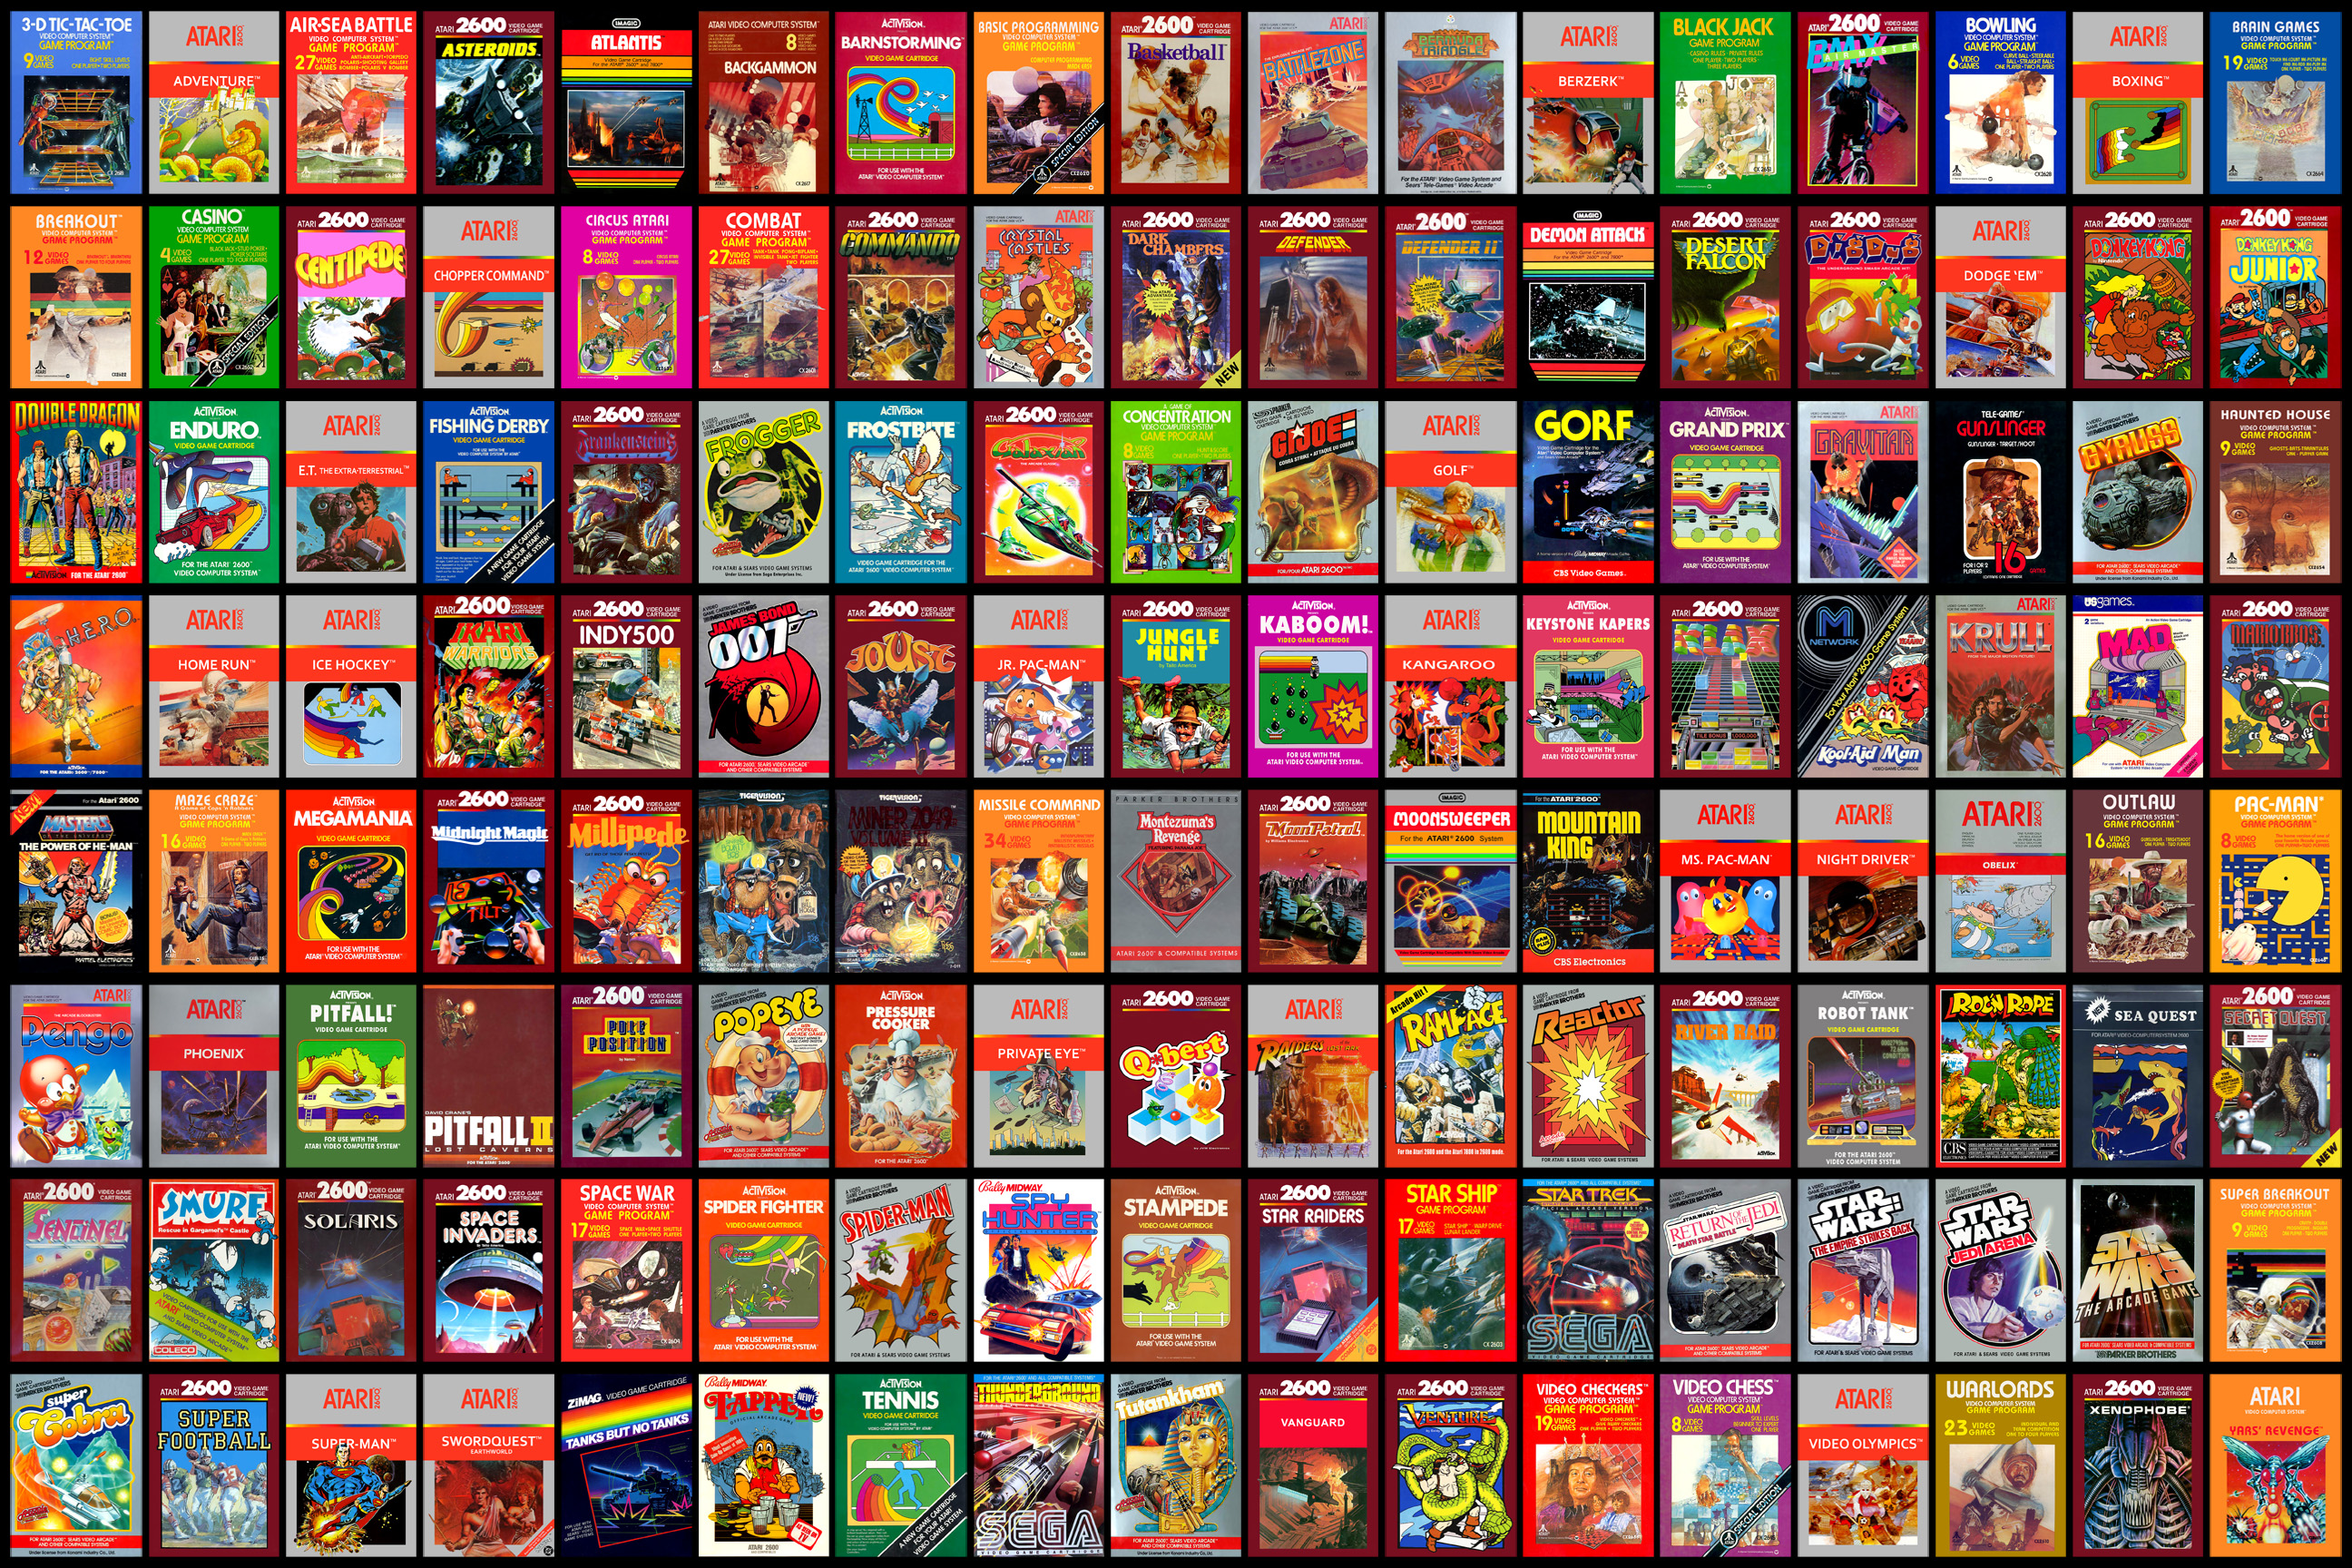
\includegraphics[width=\linewidth]{./figs/atari}
  \end{textblock*}

  \begin{textblock*}{8cm}(3cm, -0.5cm)
    
\includegraphics[width=\linewidth]{./figs/minecraft}
  \end{textblock*}

  \begin{textblock*}{2cm}(8.3cm, -2.3cm)
    {\huge Atari}
  \end{textblock*}

  \begin{textblock*}{2cm}(0cm, 3.5cm)
    {\huge Minecraft}
  \end{textblock*}
  
\end{frame}

%%%%%%%%%%%%%%%%%%%%%%%%%%%%%%%%%%%%%%%%%%%%%%%%%%%%%%%%%%%%%%%%%%%%%%%%%

\begin{frame}
  \frametitle{Challenges de la micro-gestion dans StarCraft}

  \begin{alertblock}{Contrôle de plusieurs agents en même temps}
    \begin{itemize}
    \item Actions duratives et interdépendantes.
    \item Évaluation plus chaotique des stratégies.
    \end{itemize}
  \end{alertblock}
  
  \centerline{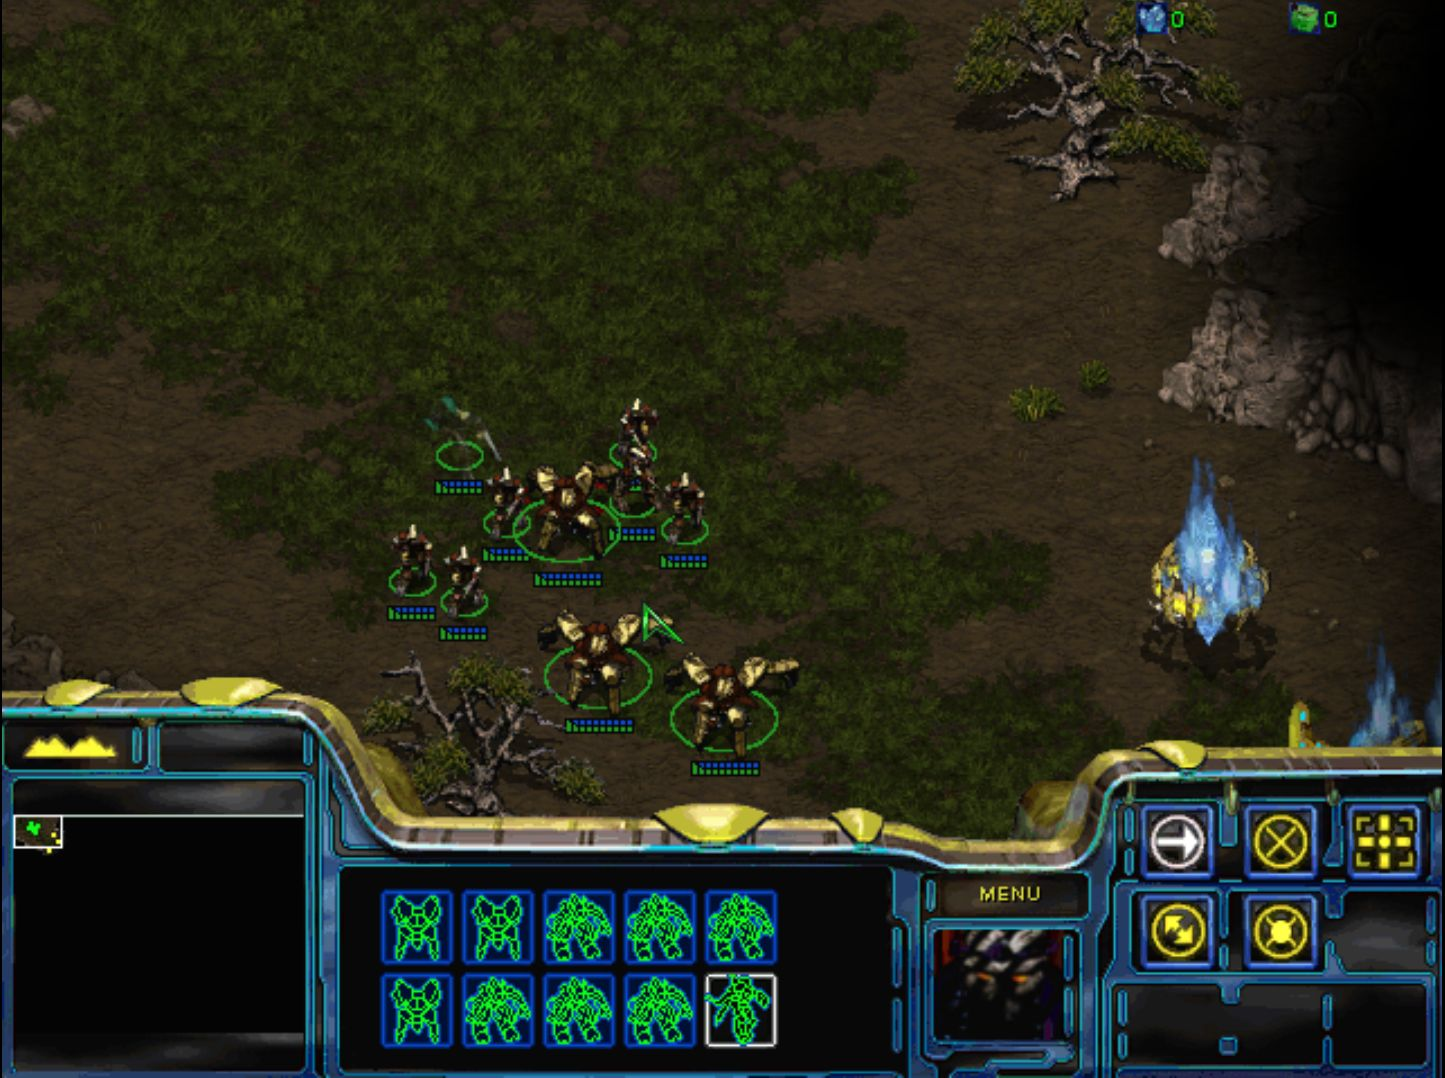
\includegraphics[width=0.7\linewidth]{./figs/starcraft_group}}  
    
\end{frame}

%%%%%%%%%%%%%%%%%%%%%%%%%%%%%%%%%%%%%%%%%%%%%%%%%%%%%%%%%%%%%%%%%%%%%%%%%

\begin{frame}
  \frametitle{Challenges de la micro-gestion dans StarCraft}

  \begin{alertblock}{Explorer en tirant au hasard une action casse tout équilibre}
    \begin{itemize}
    \item Désorganisation des agents.
    \item Défaite assuré dont aucune leçon ne peut être tirée.
    \end{itemize}
  \end{alertblock}

  \centerline{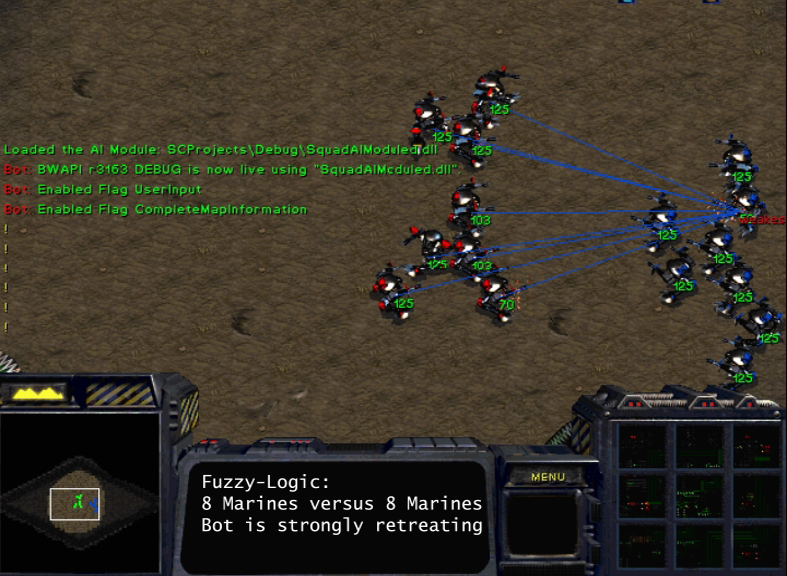
\includegraphics[width=0.7\linewidth]{./figs/starcraft_squad}}  
    
\end{frame}

%%%%%%%%%%%%%%%%%%%%%%%%%%%%%%%%%%%%%%%%%%%%%%%%%%%%%%%%%%%%%%%%%%%%%%%%%

\section{Scénarii de micro-gestion}

\begin{frame}
  \frametitle{Scénarii de micro-gestion}

  \begin{textblock*}{5cm}(0cm, -3cm)
    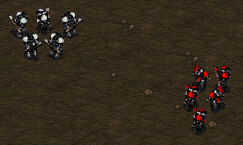
\includegraphics[width=\linewidth]{./figs/starcraft_m5v5}
  \end{textblock*}

  \begin{textblock*}{5cm}(6cm, -3cm)
    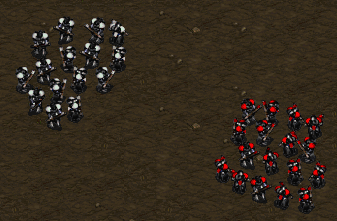
\includegraphics[width=0.9\linewidth]{./figs/starcraft_m15v16}
  \end{textblock*}

  \begin{textblock*}{5cm}(0cm, 1cm)
    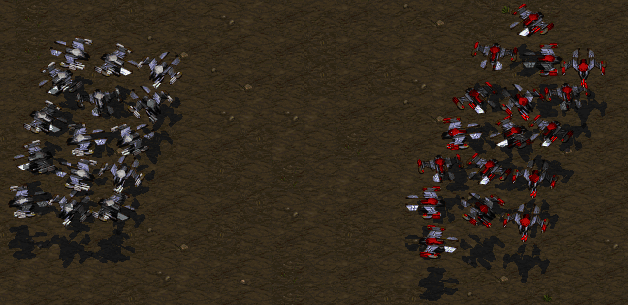
\includegraphics[width=\linewidth]{./figs/starcraft_w15v17}
  \end{textblock*}

  \begin{textblock*}{5cm}(6cm, 1cm)
    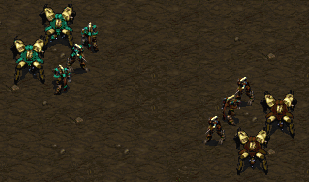
\includegraphics[width=0.9\linewidth]{./figs/starcraft_mix_dragoon_zealot}
  \end{textblock*}

  \begin{textblock*}{5cm}(0cm, 0cm)
    5 marines vs 5 (m5v5)
  \end{textblock*}

  \begin{textblock*}{5cm}(6cm, 0cm)
    15 marines vs 16 (m15v16)
  \end{textblock*}

  \begin{textblock*}{5cm}(0cm, 3.5cm)
    15 wraith vs 17 (w15v17)
  \end{textblock*}

  \begin{textblock*}{5cm}(6cm, 3.8cm)
    mix 3 zealots + 2 dragoons
  \end{textblock*}

\end{frame}

%%%%%%%%%%%%%%%%%%%%%%%%%%%%%%%%%%%%%%%%%%%%%%%%%%%%%%%%%%%%%%%%%%%%%%%%%

\section{Algos d'apprentissage par renforcement}

\begin{frame}
  \frametitle{Le modèle MDP de base}

  \begin{textblock*}{8.25cm}(1.3cm, -2cm)
    \centerline{\def\svgwidth{\columnwidth}%LaTeX with PSTricks extensions
%%Creator: inkscape 0.91
%%Please note this file requires PSTricks extensions
\psset{xunit=.5pt,yunit=.5pt,runit=.5pt}
\begin{pspicture}(541.9329834,123.85713959)
{
\newrgbcolor{curcolor}{0 0 0}
\pscustom[linewidth=1,linecolor=curcolor]
{
\newpath
\moveto(168.2601989,61.92856959)
\curveto(168.2601989,28.01999959)(140.7401989,0.49999959)(106.8316289,0.49999959)
\curveto(72.9230589,0.49999959)(45.4030589,28.01999959)(45.4030589,61.92856959)
\curveto(45.4030589,95.83714959)(72.9230589,123.35713959)(106.8316289,123.35713959)
\curveto(140.7401989,123.35713959)(168.2601989,95.83714959)(168.2601989,61.92856959)
\closepath
}
}
{
\newrgbcolor{curcolor}{0 0 0}
\pscustom[linestyle=none,fillstyle=solid,fillcolor=curcolor]
{
\newpath
\moveto(89.42440595,63.71080075)
\curveto(89.84758303,63.56757158)(90.25773928,63.261582)(90.6548747,62.792832)
\curveto(91.05852053,62.324082)(91.46216636,61.67955075)(91.8658122,60.85923825)
\lineto(93.86776532,56.87486325)
\lineto(91.7486247,56.87486325)
\lineto(89.88339032,60.61509762)
\curveto(89.40161949,61.59166012)(88.93286949,62.23944658)(88.47714032,62.558457)
\curveto(88.02792157,62.87746742)(87.4126872,63.03697262)(86.6314372,63.03697262)
\lineto(84.4829997,63.03697262)
\lineto(84.4829997,56.87486325)
\lineto(82.51034345,56.87486325)
\lineto(82.51034345,71.45494137)
\lineto(86.96346845,71.45494137)
\curveto(88.63013511,71.45494137)(89.8736247,71.10663408)(90.6939372,70.4100195)
\curveto(91.5142497,69.71340492)(91.92440595,68.66197262)(91.92440595,67.25572262)
\curveto(91.92440595,66.33775387)(91.7095622,65.57603512)(91.2798747,64.97056637)
\curveto(90.85669761,64.36509762)(90.23820803,63.94517575)(89.42440595,63.71080075)
\closepath
\moveto(84.4829997,69.83384762)
\lineto(84.4829997,64.65806637)
\lineto(86.96346845,64.65806637)
\curveto(87.91398928,64.65806637)(88.63013511,64.87616533)(89.11190595,65.31236325)
\curveto(89.6001872,65.75507158)(89.84432782,66.40285804)(89.84432782,67.25572262)
\curveto(89.84432782,68.10858721)(89.6001872,68.74986325)(89.11190595,69.17955075)
\curveto(88.63013511,69.61574867)(87.91398928,69.83384762)(86.96346845,69.83384762)
\lineto(84.4829997,69.83384762)
\closepath
}
}
{
\newrgbcolor{curcolor}{0 0 0}
\pscustom[linestyle=none,fillstyle=solid,fillcolor=curcolor]
{
\newpath
\moveto(100.89901532,62.37291012)
\curveto(99.4471924,62.37291012)(98.44133303,62.2068945)(97.8814372,61.87486325)
\curveto(97.32154136,61.542832)(97.04159345,60.97642575)(97.04159345,60.1756445)
\curveto(97.04159345,59.53762367)(97.24992678,59.02981117)(97.66659345,58.652207)
\curveto(98.08977053,58.28111325)(98.6626872,58.09556637)(99.38534345,58.09556637)
\curveto(100.3814372,58.09556637)(101.17896324,58.44712887)(101.77792157,59.15025387)
\curveto(102.38339032,59.85988929)(102.6861247,60.8006445)(102.6861247,61.9725195)
\lineto(102.6861247,62.37291012)
\lineto(100.89901532,62.37291012)
\closepath
\moveto(104.4829997,63.11509762)
\lineto(104.4829997,56.87486325)
\lineto(102.6861247,56.87486325)
\lineto(102.6861247,58.5350195)
\curveto(102.27596845,57.870957)(101.76490074,57.37942054)(101.15292157,57.06041012)
\curveto(100.5409424,56.74791012)(99.79224449,56.59166012)(98.90682782,56.59166012)
\curveto(97.78703615,56.59166012)(96.89510907,56.90416012)(96.23104657,57.52916012)
\curveto(95.57349449,58.16067054)(95.24471845,59.0037695)(95.24471845,60.058457)
\curveto(95.24471845,61.28892575)(95.6548747,62.21666012)(96.4751872,62.84166012)
\curveto(97.30201011,63.46666012)(98.53247886,63.77916012)(100.16659345,63.77916012)
\lineto(102.6861247,63.77916012)
\lineto(102.6861247,63.95494137)
\curveto(102.6861247,64.78176429)(102.4126872,65.41978512)(101.8658122,65.86900387)
\curveto(101.32544761,66.32473304)(100.56372886,66.55259762)(99.58065595,66.55259762)
\curveto(98.95565595,66.55259762)(98.34693199,66.47772783)(97.75448407,66.32798825)
\curveto(97.16203615,66.17824867)(96.5923747,65.95363929)(96.0454997,65.65416012)
\lineto(96.0454997,67.31431637)
\curveto(96.70305178,67.56822262)(97.34107261,67.75702471)(97.9595622,67.88072262)
\curveto(98.57805178,68.01093096)(99.18026532,68.07603512)(99.76620282,68.07603512)
\curveto(101.34823407,68.07603512)(102.5298747,67.66587887)(103.3111247,66.84556637)
\curveto(104.0923747,66.02525387)(104.4829997,64.78176429)(104.4829997,63.11509762)
\closepath
}
}
{
\newrgbcolor{curcolor}{0 0 0}
\pscustom[linestyle=none,fillstyle=solid,fillcolor=curcolor]
{
\newpath
\moveto(108.21346845,67.81236325)
\lineto(110.01034345,67.81236325)
\lineto(110.01034345,56.87486325)
\lineto(108.21346845,56.87486325)
\lineto(108.21346845,67.81236325)
\closepath
\moveto(108.21346845,72.07017575)
\lineto(110.01034345,72.07017575)
\lineto(110.01034345,69.79478512)
\lineto(108.21346845,69.79478512)
\lineto(108.21346845,72.07017575)
\closepath
}
}
{
\newrgbcolor{curcolor}{0 0 0}
\pscustom[linestyle=none,fillstyle=solid,fillcolor=curcolor]
{
\newpath
\moveto(122.85214032,63.47642575)
\lineto(122.85214032,56.87486325)
\lineto(121.05526532,56.87486325)
\lineto(121.05526532,63.417832)
\curveto(121.05526532,64.45298825)(120.8534424,65.22772783)(120.44979657,65.74205075)
\curveto(120.04615074,66.25637367)(119.44068199,66.51353512)(118.63339032,66.51353512)
\curveto(117.66333824,66.51353512)(116.89836428,66.20429033)(116.33846845,65.58580075)
\curveto(115.77857261,64.96731117)(115.4986247,64.12421221)(115.4986247,63.05650387)
\lineto(115.4986247,56.87486325)
\lineto(113.69198407,56.87486325)
\lineto(113.69198407,67.81236325)
\lineto(115.4986247,67.81236325)
\lineto(115.4986247,66.1131445)
\curveto(115.9283122,66.77069658)(116.43286949,67.26223304)(117.01229657,67.58775387)
\curveto(117.59823407,67.91327471)(118.2720622,68.07603512)(119.03378095,68.07603512)
\curveto(120.29029136,68.07603512)(121.2408122,67.68541012)(121.88534345,66.90416012)
\curveto(122.5298747,66.12942054)(122.85214032,64.98684242)(122.85214032,63.47642575)
\closepath
}
}
{
\newrgbcolor{curcolor}{0 0 0}
\pscustom[linestyle=none,fillstyle=solid,fillcolor=curcolor]
{
\newpath
\moveto(131.0064372,55.85923825)
\curveto(130.4986247,54.55715492)(130.00383303,53.70754554)(129.5220622,53.31041012)
\curveto(129.04029136,52.91327471)(128.39576011,52.714707)(127.58846845,52.714707)
\lineto(126.15292157,52.714707)
\lineto(126.15292157,54.21861325)
\lineto(127.20760907,54.21861325)
\curveto(127.70240074,54.21861325)(128.08651532,54.33580075)(128.35995282,54.57017575)
\curveto(128.63339032,54.80455075)(128.9361247,55.35793617)(129.26815595,56.230332)
\lineto(129.59042157,57.0506445)
\lineto(125.16659345,67.81236325)
\lineto(127.07089032,67.81236325)
\lineto(130.48885907,59.25767575)
\lineto(133.90682782,67.81236325)
\lineto(135.8111247,67.81236325)
\lineto(131.0064372,55.85923825)
\closepath
}
}
{
\newrgbcolor{curcolor}{0 0 0}
\pscustom[linewidth=1,linecolor=curcolor]
{
\newpath
\moveto(492.37173,61.92856959)
\curveto(492.37173,28.01999959)(464.85173,0.49999959)(430.94316,0.49999959)
\curveto(397.03459,0.49999959)(369.51459,28.01999959)(369.51459,61.92856959)
\curveto(369.51459,95.83714959)(397.03459,123.35713959)(430.94316,123.35713959)
\curveto(464.85173,123.35713959)(492.37173,95.83714959)(492.37173,61.92856959)
\closepath
}
}
{
\newrgbcolor{curcolor}{0 0 0}
\pscustom[linestyle=none,fillstyle=solid,fillcolor=curcolor]
{
\newpath
\moveto(412.90605423,70.85435544)
\lineto(412.90605423,68.93052731)
\curveto(412.15735632,69.28860023)(411.45097611,69.55552731)(410.78691361,69.73130856)
\curveto(410.12285111,69.90708981)(409.48157507,69.99498044)(408.86308548,69.99498044)
\curveto(407.78886673,69.99498044)(406.95878861,69.7866471)(406.37285111,69.36998044)
\curveto(405.79342403,68.95331377)(405.50371048,68.36086585)(405.50371048,67.59263669)
\curveto(405.50371048,66.94810544)(405.69576778,66.45982419)(406.07988236,66.12779294)
\curveto(406.47050736,65.8022721)(407.20618444,65.53860023)(408.28691361,65.33677731)
\lineto(409.47831986,65.09263669)
\curveto(410.94967403,64.81268877)(412.0336584,64.3178971)(412.73027298,63.60826169)
\curveto(413.43339798,62.90513669)(413.78496048,61.96112627)(413.78496048,60.77623044)
\curveto(413.78496048,59.36347002)(413.30970007,58.29250648)(412.35917923,57.56333981)
\curveto(411.41516882,56.83417315)(410.02845007,56.46958981)(408.19902298,56.46958981)
\curveto(407.50891882,56.46958981)(406.77324173,56.54771481)(405.99199173,56.70396481)
\curveto(405.21725215,56.86021481)(404.41321569,57.0913346)(403.57988236,57.39732419)
\lineto(403.57988236,59.42857419)
\curveto(404.38066361,58.97935544)(405.16516882,58.64081377)(405.93339798,58.41294919)
\curveto(406.70162715,58.1850846)(407.45683548,58.07115231)(408.19902298,58.07115231)
\curveto(409.32532507,58.07115231)(410.19446569,58.29250648)(410.80644486,58.73521481)
\curveto(411.41842403,59.17792315)(411.72441361,59.80943356)(411.72441361,60.62974606)
\curveto(411.72441361,61.3458919)(411.50305944,61.90578773)(411.06035111,62.30943356)
\curveto(410.62415319,62.7130794)(409.90475215,63.01581377)(408.90214798,63.21763669)
\lineto(407.70097611,63.45201169)
\curveto(406.22962194,63.74498044)(405.16516882,64.20396481)(404.50761673,64.82896481)
\curveto(403.85006465,65.45396481)(403.52128861,66.32310544)(403.52128861,67.43638669)
\curveto(403.52128861,68.72544919)(403.97376257,69.74107419)(404.87871048,70.48326169)
\curveto(405.79016882,71.22544919)(407.04342403,71.59654294)(408.63847611,71.59654294)
\curveto(409.32206986,71.59654294)(410.01868444,71.53469398)(410.72831986,71.41099606)
\curveto(411.43795528,71.28729815)(412.16386673,71.10175127)(412.90605423,70.85435544)
\closepath
}
}
{
\newrgbcolor{curcolor}{0 0 0}
\pscustom[linestyle=none,fillstyle=solid,fillcolor=curcolor]
{
\newpath
\moveto(416.59746048,61.06919919)
\lineto(416.59746048,67.69029294)
\lineto(418.39433548,67.69029294)
\lineto(418.39433548,61.13755856)
\curveto(418.39433548,60.10240231)(418.5961584,59.32440752)(418.99980423,58.80357419)
\curveto(419.40345007,58.28925127)(420.00891882,58.03208981)(420.81621048,58.03208981)
\curveto(421.78626257,58.03208981)(422.55123653,58.3413346)(423.11113236,58.95982419)
\curveto(423.67753861,59.57831377)(423.96074173,60.42141273)(423.96074173,61.48912106)
\lineto(423.96074173,67.69029294)
\lineto(425.75761673,67.69029294)
\lineto(425.75761673,56.75279294)
\lineto(423.96074173,56.75279294)
\lineto(423.96074173,58.43248044)
\curveto(423.52454382,57.76841794)(423.01673132,57.27362627)(422.43730423,56.94810544)
\curveto(421.86438757,56.62909502)(421.19706986,56.46958981)(420.43535111,56.46958981)
\curveto(419.17884069,56.46958981)(418.22506465,56.86021481)(417.57402298,57.64146481)
\curveto(416.92298132,58.42271481)(416.59746048,59.56529294)(416.59746048,61.06919919)
\closepath
}
}
{
\newrgbcolor{curcolor}{0 0 0}
\pscustom[linestyle=none,fillstyle=solid,fillcolor=curcolor]
{
\newpath
\moveto(438.57011673,63.35435544)
\lineto(438.57011673,56.75279294)
\lineto(436.77324173,56.75279294)
\lineto(436.77324173,63.29576169)
\curveto(436.77324173,64.33091794)(436.57141882,65.10565752)(436.16777298,65.61998044)
\curveto(435.76412715,66.13430335)(435.1586584,66.39146481)(434.35136673,66.39146481)
\curveto(433.38131465,66.39146481)(432.61634069,66.08222002)(432.05644486,65.46373044)
\curveto(431.49654903,64.84524085)(431.21660111,64.0021419)(431.21660111,62.93443356)
\lineto(431.21660111,56.75279294)
\lineto(429.40996048,56.75279294)
\lineto(429.40996048,67.69029294)
\lineto(431.21660111,67.69029294)
\lineto(431.21660111,65.99107419)
\curveto(431.64628861,66.64862627)(432.1508459,67.14016273)(432.73027298,67.46568356)
\curveto(433.31621048,67.7912044)(433.99003861,67.95396481)(434.75175736,67.95396481)
\curveto(436.00826778,67.95396481)(436.95878861,67.56333981)(437.60331986,66.78208981)
\curveto(438.24785111,66.00735023)(438.57011673,64.8647721)(438.57011673,63.35435544)
\closepath
}
}
{
\newrgbcolor{curcolor}{0 0 0}
\pscustom[linestyle=none,fillstyle=solid,fillcolor=curcolor]
{
\newpath
\moveto(451.26542923,63.35435544)
\lineto(451.26542923,56.75279294)
\lineto(449.46855423,56.75279294)
\lineto(449.46855423,63.29576169)
\curveto(449.46855423,64.33091794)(449.26673132,65.10565752)(448.86308548,65.61998044)
\curveto(448.45943965,66.13430335)(447.8539709,66.39146481)(447.04667923,66.39146481)
\curveto(446.07662715,66.39146481)(445.31165319,66.08222002)(444.75175736,65.46373044)
\curveto(444.19186153,64.84524085)(443.91191361,64.0021419)(443.91191361,62.93443356)
\lineto(443.91191361,56.75279294)
\lineto(442.10527298,56.75279294)
\lineto(442.10527298,67.69029294)
\lineto(443.91191361,67.69029294)
\lineto(443.91191361,65.99107419)
\curveto(444.34160111,66.64862627)(444.8461584,67.14016273)(445.42558548,67.46568356)
\curveto(446.01152298,67.7912044)(446.68535111,67.95396481)(447.44706986,67.95396481)
\curveto(448.70358028,67.95396481)(449.65410111,67.56333981)(450.29863236,66.78208981)
\curveto(450.94316361,66.00735023)(451.26542923,64.8647721)(451.26542923,63.35435544)
\closepath
}
}
{
\newrgbcolor{curcolor}{0 0 0}
\pscustom[linestyle=none,fillstyle=solid,fillcolor=curcolor]
{
\newpath
\moveto(459.41972611,55.73716794)
\curveto(458.91191361,54.4350846)(458.41712194,53.58547523)(457.93535111,53.18833981)
\curveto(457.45358028,52.7912044)(456.80904903,52.59263669)(456.00175736,52.59263669)
\lineto(454.56621048,52.59263669)
\lineto(454.56621048,54.09654294)
\lineto(455.62089798,54.09654294)
\curveto(456.11568965,54.09654294)(456.49980423,54.21373044)(456.77324173,54.44810544)
\curveto(457.04667923,54.68248044)(457.34941361,55.23586585)(457.68144486,56.10826169)
\lineto(458.00371048,56.92857419)
\lineto(453.57988236,67.69029294)
\lineto(455.48417923,67.69029294)
\lineto(458.90214798,59.13560544)
\lineto(462.32011673,67.69029294)
\lineto(464.22441361,67.69029294)
\lineto(459.41972611,55.73716794)
\closepath
}
}
{
\newrgbcolor{curcolor}{0 0 0}
\pscustom[linewidth=1.00000001,linecolor=curcolor]
{
\newpath
\moveto(52.65086078,31.12458331)
\curveto(40.69458074,20.50727774)(22.66264341,20.59296763)(10.80781045,31.32342639)
\curveto(-1.04702252,42.05388516)(-2.92323486,59.98815219)(6.45406597,72.93983312)
\curveto(15.8313668,85.89151405)(33.45514042,89.70736391)(47.34997378,81.79449996)
}
}
{
\newrgbcolor{curcolor}{0 0 0}
\pscustom[linestyle=none,fillstyle=solid,fillcolor=curcolor]
{
\newpath
\moveto(38.66026683,86.74313569)
\lineto(33.20492975,85.2467072)
\lineto(47.34997378,81.79449996)
\lineto(37.16383834,92.19847277)
\lineto(38.66026683,86.74313569)
\closepath
}
}
{
\newrgbcolor{curcolor}{0 0 0}
\pscustom[linewidth=1.00000001,linecolor=curcolor]
{
\newpath
\moveto(38.66026683,86.74313569)
\lineto(33.20492975,85.2467072)
\lineto(47.34997378,81.79449996)
\lineto(37.16383834,92.19847277)
\lineto(38.66026683,86.74313569)
\closepath
}
}
{
\newrgbcolor{curcolor}{0 0 0}
\pscustom[linewidth=1.00000001,linecolor=curcolor]
{
\newpath
\moveto(489.28210622,79.34501587)
\curveto(501.23838626,89.96232143)(519.27032359,89.87663155)(531.12515655,79.14617278)
\curveto(542.97998952,68.41571402)(544.85620186,50.48144699)(535.47890103,37.52976605)
\curveto(526.1016002,24.57808512)(508.47782658,20.76223527)(494.58299322,28.67509922)
}
}
{
\newrgbcolor{curcolor}{0 0 0}
\pscustom[linestyle=none,fillstyle=solid,fillcolor=curcolor]
{
\newpath
\moveto(503.27270017,23.72646348)
\lineto(508.72803725,25.22289197)
\lineto(494.58299322,28.67509922)
\lineto(504.76912866,18.27112641)
\lineto(503.27270017,23.72646348)
\closepath
}
}
{
\newrgbcolor{curcolor}{0 0 0}
\pscustom[linewidth=1.00000001,linecolor=curcolor]
{
\newpath
\moveto(503.27270017,23.72646348)
\lineto(508.72803725,25.22289197)
\lineto(494.58299322,28.67509922)
\lineto(504.76912866,18.27112641)
\lineto(503.27270017,23.72646348)
\closepath
}
}
{
\newrgbcolor{curcolor}{0 0 0}
\pscustom[linestyle=none,fillstyle=solid,fillcolor=curcolor]
{
\newpath
\moveto(24.88554291,43.45310383)
\curveto(24.07304291,43.45310383)(23.46106374,43.05206216)(23.04960541,42.24997883)
\curveto(22.64335541,41.45310383)(22.44023041,40.25258299)(22.44023041,38.64841633)
\curveto(22.44023041,37.04945799)(22.64335541,35.84893716)(23.04960541,35.04685383)
\curveto(23.46106374,34.24997883)(24.07304291,33.85154133)(24.88554291,33.85154133)
\curveto(25.70325124,33.85154133)(26.31523041,34.24997883)(26.72148041,35.04685383)
\curveto(27.13293874,35.84893716)(27.33866791,37.04945799)(27.33866791,38.64841633)
\curveto(27.33866791,40.25258299)(27.13293874,41.45310383)(26.72148041,42.24997883)
\curveto(26.31523041,43.05206216)(25.70325124,43.45310383)(24.88554291,43.45310383)
\closepath
\moveto(24.88554291,44.70310383)
\curveto(26.19283458,44.70310383)(27.19023041,44.18487466)(27.87773041,43.14841633)
\curveto(28.57043874,42.11716633)(28.91679291,40.61716633)(28.91679291,38.64841633)
\curveto(28.91679291,36.68487466)(28.57043874,35.18487466)(27.87773041,34.14841633)
\curveto(27.19023041,33.11716633)(26.19283458,32.60154133)(24.88554291,32.60154133)
\curveto(23.57825124,32.60154133)(22.57825124,33.11716633)(21.88554291,34.14841633)
\curveto(21.19804291,35.18487466)(20.85429291,36.68487466)(20.85429291,38.64841633)
\curveto(20.85429291,40.61716633)(21.19804291,42.11716633)(21.88554291,43.14841633)
\curveto(22.57825124,44.18487466)(23.57825124,44.70310383)(24.88554291,44.70310383)
\closepath
}
}
{
\newrgbcolor{curcolor}{0 0 0}
\pscustom[linestyle=none,fillstyle=solid,fillcolor=curcolor]
{
\newpath
\moveto(31.69804291,34.81247883)
\lineto(33.34648041,34.81247883)
\lineto(33.34648041,32.82810383)
\lineto(31.69804291,32.82810383)
\lineto(31.69804291,34.81247883)
\closepath
}
}
{
\newrgbcolor{curcolor}{0 0 0}
\pscustom[linestyle=none,fillstyle=solid,fillcolor=curcolor]
{
\newpath
\moveto(36.39335541,44.49216633)
\lineto(43.89335541,44.49216633)
\lineto(43.89335541,43.82029133)
\lineto(39.65898041,32.82810383)
\lineto(38.01054291,32.82810383)
\lineto(41.99491791,43.16404133)
\lineto(36.39335541,43.16404133)
\lineto(36.39335541,44.49216633)
\closepath
}
}
{
\newrgbcolor{curcolor}{0 0 0}
\pscustom[linestyle=none,fillstyle=solid,fillcolor=curcolor]
{
\newpath
\moveto(507.29838471,47.35599689)
\curveto(506.48588471,47.35599689)(505.87390554,46.95495523)(505.46244721,46.15287189)
\curveto(505.05619721,45.35599689)(504.85307221,44.15547606)(504.85307221,42.55130939)
\curveto(504.85307221,40.95235106)(505.05619721,39.75183023)(505.46244721,38.94974689)
\curveto(505.87390554,38.15287189)(506.48588471,37.75443439)(507.29838471,37.75443439)
\curveto(508.11609304,37.75443439)(508.72807221,38.15287189)(509.13432221,38.94974689)
\curveto(509.54578054,39.75183023)(509.75150971,40.95235106)(509.75150971,42.55130939)
\curveto(509.75150971,44.15547606)(509.54578054,45.35599689)(509.13432221,46.15287189)
\curveto(508.72807221,46.95495523)(508.11609304,47.35599689)(507.29838471,47.35599689)
\closepath
\moveto(507.29838471,48.60599689)
\curveto(508.60567637,48.60599689)(509.60307221,48.08776773)(510.29057221,47.05130939)
\curveto(510.98328054,46.02005939)(511.32963471,44.52005939)(511.32963471,42.55130939)
\curveto(511.32963471,40.58776773)(510.98328054,39.08776773)(510.29057221,38.05130939)
\curveto(509.60307221,37.02005939)(508.60567637,36.50443439)(507.29838471,36.50443439)
\curveto(505.99109304,36.50443439)(504.99109304,37.02005939)(504.29838471,38.05130939)
\curveto(503.61088471,39.08776773)(503.26713471,40.58776773)(503.26713471,42.55130939)
\curveto(503.26713471,44.52005939)(503.61088471,46.02005939)(504.29838471,47.05130939)
\curveto(504.99109304,48.08776773)(505.99109304,48.60599689)(507.29838471,48.60599689)
\closepath
}
}
{
\newrgbcolor{curcolor}{0 0 0}
\pscustom[linestyle=none,fillstyle=solid,fillcolor=curcolor]
{
\newpath
\moveto(514.11088471,38.71537189)
\lineto(515.75932221,38.71537189)
\lineto(515.75932221,36.73099689)
\lineto(514.11088471,36.73099689)
\lineto(514.11088471,38.71537189)
\closepath
}
}
{
\newrgbcolor{curcolor}{0 0 0}
\pscustom[linestyle=none,fillstyle=solid,fillcolor=curcolor]
{
\newpath
\moveto(522.77494721,43.19193439)
\curveto(522.06661387,43.19193439)(521.50411387,42.94974689)(521.08744721,42.46537189)
\curveto(520.67598887,41.98099689)(520.47025971,41.31693439)(520.47025971,40.47318439)
\curveto(520.47025971,39.63464273)(520.67598887,38.97058023)(521.08744721,38.48099689)
\curveto(521.50411387,37.99662189)(522.06661387,37.75443439)(522.77494721,37.75443439)
\curveto(523.48328054,37.75443439)(524.04317637,37.99662189)(524.45463471,38.48099689)
\curveto(524.87130137,38.97058023)(525.07963471,39.63464273)(525.07963471,40.47318439)
\curveto(525.07963471,41.31693439)(524.87130137,41.98099689)(524.45463471,42.46537189)
\curveto(524.04317637,42.94974689)(523.48328054,43.19193439)(522.77494721,43.19193439)
\closepath
\moveto(525.90775971,48.13724689)
\lineto(525.90775971,46.69974689)
\curveto(525.51192637,46.88724689)(525.11088471,47.03047606)(524.70463471,47.12943439)
\curveto(524.30359304,47.22839273)(523.90515554,47.27787189)(523.50932221,47.27787189)
\curveto(522.46765554,47.27787189)(521.67078054,46.92630939)(521.11869721,46.22318439)
\curveto(520.57182221,45.52005939)(520.25932221,44.45755939)(520.18119721,43.03568439)
\curveto(520.48848887,43.48880939)(520.87390554,43.83516356)(521.33744721,44.07474689)
\curveto(521.80098887,44.31953856)(522.31140554,44.44193439)(522.86869721,44.44193439)
\curveto(524.04057221,44.44193439)(524.96505137,44.08516356)(525.64213471,43.37162189)
\curveto(526.32442637,42.66328856)(526.66557221,41.69714273)(526.66557221,40.47318439)
\curveto(526.66557221,39.27526773)(526.31140554,38.31433023)(525.60307221,37.59037189)
\curveto(524.89473887,36.86641356)(523.95203054,36.50443439)(522.77494721,36.50443439)
\curveto(521.42598887,36.50443439)(520.39473887,37.02005939)(519.68119721,38.05130939)
\curveto(518.96765554,39.08776773)(518.61088471,40.58776773)(518.61088471,42.55130939)
\curveto(518.61088471,44.39505939)(519.04838471,45.86380939)(519.92338471,46.95755939)
\curveto(520.79838471,48.05651773)(521.97286387,48.60599689)(523.44682221,48.60599689)
\curveto(523.84265554,48.60599689)(524.24109304,48.56693439)(524.64213471,48.48880939)
\curveto(525.04838471,48.41068439)(525.47025971,48.29349689)(525.90775971,48.13724689)
\closepath
}
}
{
\newrgbcolor{curcolor}{0 0 0}
\pscustom[linestyle=none,fillstyle=solid,fillcolor=curcolor]
{
\newpath
\moveto(259.06873993,105.59937458)
\curveto(258.25623993,105.59937458)(257.64426076,105.19833291)(257.23280243,104.39624958)
\curveto(256.82655243,103.59937458)(256.62342743,102.39885374)(256.62342743,100.79468708)
\curveto(256.62342743,99.19572874)(256.82655243,97.99520791)(257.23280243,97.19312458)
\curveto(257.64426076,96.39624958)(258.25623993,95.99781208)(259.06873993,95.99781208)
\curveto(259.88644826,95.99781208)(260.49842743,96.39624958)(260.90467743,97.19312458)
\curveto(261.31613576,97.99520791)(261.52186493,99.19572874)(261.52186493,100.79468708)
\curveto(261.52186493,102.39885374)(261.31613576,103.59937458)(260.90467743,104.39624958)
\curveto(260.49842743,105.19833291)(259.88644826,105.59937458)(259.06873993,105.59937458)
\closepath
\moveto(259.06873993,106.84937458)
\curveto(260.3760316,106.84937458)(261.37342743,106.33114541)(262.06092743,105.29468708)
\curveto(262.75363576,104.26343708)(263.09998993,102.76343708)(263.09998993,100.79468708)
\curveto(263.09998993,98.83114541)(262.75363576,97.33114541)(262.06092743,96.29468708)
\curveto(261.37342743,95.26343708)(260.3760316,94.74781208)(259.06873993,94.74781208)
\curveto(257.76144826,94.74781208)(256.76144826,95.26343708)(256.06873993,96.29468708)
\curveto(255.38123993,97.33114541)(255.03748993,98.83114541)(255.03748993,100.79468708)
\curveto(255.03748993,102.76343708)(255.38123993,104.26343708)(256.06873993,105.29468708)
\curveto(256.76144826,106.33114541)(257.76144826,106.84937458)(259.06873993,106.84937458)
\closepath
}
}
{
\newrgbcolor{curcolor}{0 0 0}
\pscustom[linestyle=none,fillstyle=solid,fillcolor=curcolor]
{
\newpath
\moveto(265.88123993,96.95874958)
\lineto(267.52967743,96.95874958)
\lineto(267.52967743,94.97437458)
\lineto(265.88123993,94.97437458)
\lineto(265.88123993,96.95874958)
\closepath
}
}
{
\newrgbcolor{curcolor}{0 0 0}
\pscustom[linestyle=none,fillstyle=solid,fillcolor=curcolor]
{
\newpath
\moveto(275.75623993,101.26343708)
\curveto(276.51144826,101.10197874)(277.09998993,100.76604124)(277.52186493,100.25562458)
\curveto(277.94894826,99.74520791)(278.16248993,99.11499958)(278.16248993,98.36499958)
\curveto(278.16248993,97.21395791)(277.7666566,96.32333291)(276.97498993,95.69312458)
\curveto(276.18332326,95.06291624)(275.05832326,94.74781208)(273.59998993,94.74781208)
\curveto(273.1104066,94.74781208)(272.60519826,94.79729124)(272.08436493,94.89624958)
\curveto(271.56873993,94.98999958)(271.03488576,95.13322874)(270.48280243,95.32593708)
\lineto(270.48280243,96.84937458)
\curveto(270.92030243,96.59416624)(271.3994691,96.40145791)(271.92030243,96.27124958)
\curveto(272.44113576,96.14104124)(272.9854066,96.07593708)(273.55311493,96.07593708)
\curveto(274.54269826,96.07593708)(275.29530243,96.27124958)(275.81092743,96.66187458)
\curveto(276.33176076,97.05249958)(276.59217743,97.62020791)(276.59217743,98.36499958)
\curveto(276.59217743,99.05249958)(276.34998993,99.58895791)(275.86561493,99.97437458)
\curveto(275.38644826,100.36499958)(274.71717743,100.56031208)(273.85780243,100.56031208)
\lineto(272.49842743,100.56031208)
\lineto(272.49842743,101.85718708)
\lineto(273.92030243,101.85718708)
\curveto(274.6963441,101.85718708)(275.2900941,102.01083291)(275.70155243,102.31812458)
\curveto(276.11301076,102.63062458)(276.31873993,103.07854124)(276.31873993,103.66187458)
\curveto(276.31873993,104.26083291)(276.10519826,104.71916624)(275.67811493,105.03687458)
\curveto(275.25623993,105.35979124)(274.6494691,105.52124958)(273.85780243,105.52124958)
\curveto(273.42551076,105.52124958)(272.9619691,105.47437458)(272.46717743,105.38062458)
\curveto(271.97238576,105.28687458)(271.42811493,105.14104124)(270.83436493,104.94312458)
\lineto(270.83436493,106.34937458)
\curveto(271.43332326,106.51604124)(271.9932191,106.64104124)(272.51405243,106.72437458)
\curveto(273.0400941,106.80770791)(273.53488576,106.84937458)(273.99842743,106.84937458)
\curveto(275.1963441,106.84937458)(276.14426076,106.57593708)(276.84217743,106.02906208)
\curveto(277.5400941,105.48739541)(277.88905243,104.75302041)(277.88905243,103.82593708)
\curveto(277.88905243,103.18010374)(277.7041566,102.63322874)(277.33436493,102.18531208)
\curveto(276.96457326,101.74260374)(276.4385316,101.43531208)(275.75623993,101.26343708)
\closepath
}
}
{
\newrgbcolor{curcolor}{0 0 0}
\pscustom[linestyle=none,fillstyle=solid,fillcolor=curcolor]
{
\newpath
\moveto(262.38358979,57.0851839)
\curveto(261.57108979,57.0851839)(260.95911062,56.68414224)(260.54765229,55.8820589)
\curveto(260.14140229,55.0851839)(259.93827729,53.88466307)(259.93827729,52.2804964)
\curveto(259.93827729,50.68153807)(260.14140229,49.48101724)(260.54765229,48.6789339)
\curveto(260.95911062,47.8820589)(261.57108979,47.4836214)(262.38358979,47.4836214)
\curveto(263.20129812,47.4836214)(263.81327729,47.8820589)(264.21952729,48.6789339)
\curveto(264.63098562,49.48101724)(264.83671479,50.68153807)(264.83671479,52.2804964)
\curveto(264.83671479,53.88466307)(264.63098562,55.0851839)(264.21952729,55.8820589)
\curveto(263.81327729,56.68414224)(263.20129812,57.0851839)(262.38358979,57.0851839)
\closepath
\moveto(262.38358979,58.3351839)
\curveto(263.69088145,58.3351839)(264.68827729,57.81695474)(265.37577729,56.7804964)
\curveto(266.06848562,55.7492464)(266.41483979,54.2492464)(266.41483979,52.2804964)
\curveto(266.41483979,50.31695474)(266.06848562,48.81695474)(265.37577729,47.7804964)
\curveto(264.68827729,46.7492464)(263.69088145,46.2336214)(262.38358979,46.2336214)
\curveto(261.07629812,46.2336214)(260.07629812,46.7492464)(259.38358979,47.7804964)
\curveto(258.69608979,48.81695474)(258.35233979,50.31695474)(258.35233979,52.2804964)
\curveto(258.35233979,54.2492464)(258.69608979,55.7492464)(259.38358979,56.7804964)
\curveto(260.07629812,57.81695474)(261.07629812,58.3351839)(262.38358979,58.3351839)
\closepath
}
}
{
\newrgbcolor{curcolor}{0 0 0}
\pscustom[linestyle=none,fillstyle=solid,fillcolor=curcolor]
{
\newpath
\moveto(269.19608979,48.4445589)
\lineto(270.84452729,48.4445589)
\lineto(270.84452729,46.4601839)
\lineto(269.19608979,46.4601839)
\lineto(269.19608979,48.4445589)
\closepath
}
}
{
\newrgbcolor{curcolor}{0 0 0}
\pscustom[linestyle=none,fillstyle=solid,fillcolor=curcolor]
{
\newpath
\moveto(278.62577729,56.7492464)
\lineto(274.64140229,50.5226839)
\lineto(278.62577729,50.5226839)
\lineto(278.62577729,56.7492464)
\closepath
\moveto(278.21171479,58.1242464)
\lineto(280.19608979,58.1242464)
\lineto(280.19608979,50.5226839)
\lineto(281.86015229,50.5226839)
\lineto(281.86015229,49.2101839)
\lineto(280.19608979,49.2101839)
\lineto(280.19608979,46.4601839)
\lineto(278.62577729,46.4601839)
\lineto(278.62577729,49.2101839)
\lineto(273.36015229,49.2101839)
\lineto(273.36015229,50.7336214)
\lineto(278.21171479,58.1242464)
\closepath
}
}
{
\newrgbcolor{curcolor}{0 0 0}
\pscustom[linewidth=1,linecolor=curcolor]
{
\newpath
\moveto(167.92879,62.95115959)
\curveto(232.70339,93.53022959)(301.79318,95.61925959)(368.81625,68.60996959)
}
}
{
\newrgbcolor{curcolor}{0 0 0}
\pscustom[linestyle=none,fillstyle=solid,fillcolor=curcolor]
{
\newpath
\moveto(359.54106073,72.34773148)
\lineto(354.33588026,70.13276053)
\lineto(368.81625,68.60996959)
\lineto(357.32608977,77.55291194)
\lineto(359.54106073,72.34773148)
\closepath
}
}
{
\newrgbcolor{curcolor}{0 0 0}
\pscustom[linewidth=1,linecolor=curcolor]
{
\newpath
\moveto(359.54106073,72.34773148)
\lineto(354.33588026,70.13276053)
\lineto(368.81625,68.60996959)
\lineto(357.32608977,77.55291194)
\lineto(359.54106073,72.34773148)
\closepath
}
}
{
\newrgbcolor{curcolor}{0 0 0}
\pscustom[linewidth=1,linecolor=curcolor]
{
\newpath
\moveto(367.81591,66.60766959)
\curveto(302.04096,29.02618959)(225.94876,36.94059959)(166.92845,60.94885959)
}
}
{
\newrgbcolor{curcolor}{0 0 0}
\pscustom[linestyle=none,fillstyle=solid,fillcolor=curcolor]
{
\newpath
\moveto(176.1914041,57.18087852)
\lineto(181.40377817,59.37886774)
\lineto(166.92845,60.94885959)
\lineto(178.38939332,51.96850446)
\lineto(176.1914041,57.18087852)
\closepath
}
}
{
\newrgbcolor{curcolor}{0 0 0}
\pscustom[linewidth=1,linecolor=curcolor]
{
\newpath
\moveto(176.1914041,57.18087852)
\lineto(181.40377817,59.37886774)
\lineto(166.92845,60.94885959)
\lineto(178.38939332,51.96850446)
\lineto(176.1914041,57.18087852)
\closepath
}
}
\end{pspicture}
}
  \end{textblock*}

  \begin{textblock*}{8.25cm}(1.3cm, 1cm)
    \begin{block}{À chaque instant $t$}
      \begin{itemize}
      \item À l'état $s^t$, ``choisir'' l'action $a^t$.
      \item Aller à l'état $s^{t+1}$ avec la récompense $r^t$
      \end{itemize}
    \end{block}
  \end{textblock*}

  % \centerline{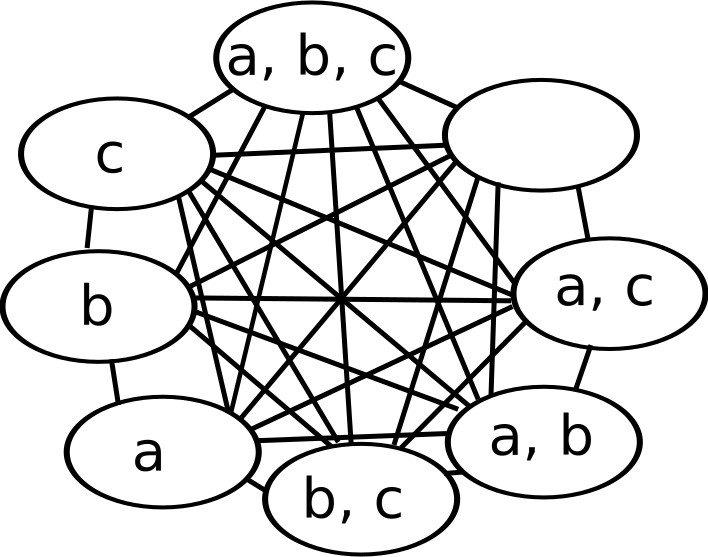
\includegraphics[width=0.9\linewidth]{./figs/mdp}}

\end{frame}

%%%%%%%%%%%%%%%%%%%%%%%%%%%%%%%%%%%%%%%%%%%%%%%%%%%%%%%%%%%%%%%%%%%%%%%%%

\begin{frame}
  \frametitle{Le modèle MDP greedy}

  \begin{textblock*}{11cm}(0cm, -3cm)
    \centerline{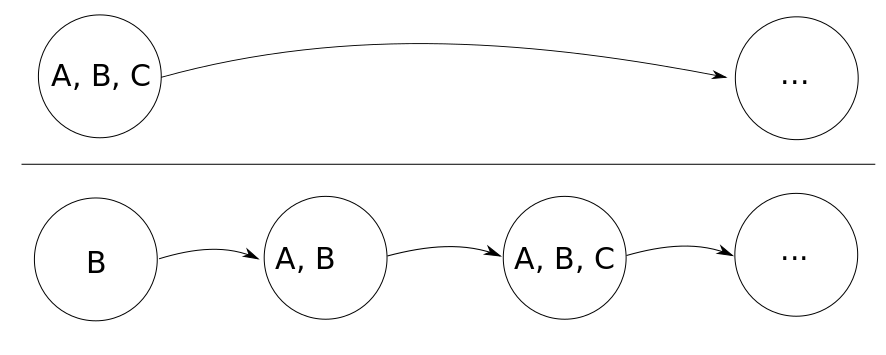
\includegraphics[width=0.9\linewidth]{./figs/chaine_markov_greedy.png}}
  \end{textblock*}
  
  \begin{textblock*}{11cm}(0cm, 1.5cm)
    \begin{exampleblock}{À chaque instant $t$}
      \begin{itemize}
      \item Créer autant d'états intermédiaires que d'unités.
      \item Chaque unité tour à tour ``choisit'' une action.
      \item Quand la dernière joue, aller à l'état suivant et recevoir
        la récompense.
      \end{itemize}
    \end{exampleblock}
  \end{textblock*}

\end{frame}

%%%%%%%%%%%%%%%%%%%%%%%%%%%%%%%%%%%%%%%%%%%%%%%%%%%%%%%%%%%%%%%%%%%%%%%%%

\begin{frame}
  \frametitle{Algorithmes d'apprentissage par renforcement}

  \begin{block}{Q-learning (DQN)}
    \begin{itemize}
    \item Off-policy
    \item Mise à jour des paramètres $\theta$ par descente de gradient :\\
      \begin{displaymath}
        \theta_{t+1}    =    \theta_t    +  \eta  \left(r^t    +    \gamma
          \operatorname*{max}\limits_{a        \in        \mathcal{A}}
          Q_{\theta_t}(s^{t+1},a)  -  Q_{\theta_t}(s^t,a^t)\right)
        \nabla_{\theta_t} Q_{\theta_t}(s^t,a^t)
      \end{displaymath}
    \item Phase d'entraînement stochastique via $\epsilon$-greedy.
    \item Phase de test déterministe.
    \end{itemize}
  \end{block}
  
\end{frame}

%%%%%%%%%%%%%%%%%%%%%%%%%%%%%%%%%%%%%%%%%%%%%%%%%%%%%%%%%%%%%%%%%%%%%%%%%

\begin{frame}
  \frametitle{Algorithmes d'apprentissage par renforcement}

  \begin{block}{REINFORCE (PG)}
    \begin{itemize}
    \item On-policy
    \item  Apprentissage   sur  les  traces  $(s^t,   a^t,  s^{t+1},
      r^{t+1})_{t=1,\ldots,T-1}$ générées
    \item Mise à jour des paramètres $\theta$ par descente de gradient :\\
      \begin{displaymath}
        \theta_{k+1}    =   \theta_k    +   \eta    \sum^T_{t=1}   R^t
        \nabla_{\theta_k} [log\ \pi_{\theta_k}(a^t \mid s^t)]
      \end{displaymath}
    \item Gibbs policy :
      \begin{displaymath}
        \pi_\theta(a              \mid               s)              =
        \frac{exp(\phi_\theta(a,s)/\tau)}{\sum_{b \in \mathcal{A}(s)}exp(\phi_\theta(b,s)/\tau)}
      \end{displaymath}
    \item $\phi_\theta$ est le réseau de neurones de paramètres $\theta$.
    \end{itemize}
  \end{block}

\end{frame}

%%%%%%%%%%%%%%%%%%%%%%%%%%%%%%%%%%%%%%%%%%%%%%%%%%%%%%%%%%%%%%%%%%%%%%%%%

\begin{frame}
  \frametitle{De l'apprentissage par renforcement sans gradient ?}

  \begin{block}{{\it Gradient-free} en mode brutasse}
    \begin{itemize}
    \item Soit une politique déterministe.
    \item Soit $R(\theta)$ sa récompense cumulative.
    \item Optimisation stochastique {\it gradient-free} :
      \begin{displaymath}
        \theta_{k+1} = \theta_k + \eta_k R(\theta_k + \delta u_k) u_k
      \end{displaymath}
      avec $u_k$ un vecteur random sur la sphère unité.
    \end{itemize}
  \end{block}

\end{frame}

%%%%%%%%%%%%%%%%%%%%%%%%%%%%%%%%%%%%%%%%%%%%%%%%%%%%%%%%%%%%%%%%%%%%%%%%%

\begin{frame}
  \frametitle{L'intuition derrière une optimisation {\it gradient-free}}

  \begin{exampleblock}{L'idée}
    \begin{itemize}
    \item  Sans  aléatoire,  pas   d'exploration  avec  une  politique
      déterministe.
    \item On  ajoute donc  du bruit $\delta  u_k$ dans  les paramètres
      $\theta$.
    \end{itemize}    
  \end{exampleblock}

  \uncover<2->
  {
    \begin{block}{Passage d'un problème d'exploration à un autre}
      Espace d'action $\Rightarrow$ Espace de politique
    \end{block}
  }
  
  \uncover<3>
  {
    \begin{alertblock}{Problème}
      \begin{itemize}
      \item Dans  un deep NN,  il y a trop  de paramètres $\theta$  : ce
        n'est pas gérable !
      \item Donc on ne fait ça que pour la dernière couche du NN.
      \end{itemize}    
    \end{alertblock}
  }

\end{frame}

%%%%%%%%%%%%%%%%%%%%%%%%%%%%%%%%%%%%%%%%%%%%%%%%%%%%%%%%%%%%%%%%%%%%%%%%%

\section{Features et modèle}

\begin{frame}
  \frametitle{Le modèle}

  \begin{block}{Les inputs}
    \begin{itemize}
    \item Matrice où chaque ligne représente une unité.
    \item 17 features par unité : camp, type, HP, $\ldots$ + 9 distances
    \end{itemize}
  \end{block}
  
\end{frame}

%%%%%%%%%%%%%%%%%%%%%%%%%%%%%%%%%%%%%%%%%%%%%%%%%%%%%%%%%%%%%%%%%%%%%%%%%

\begin{frame}
  \frametitle{Le modèle}

  \centerline{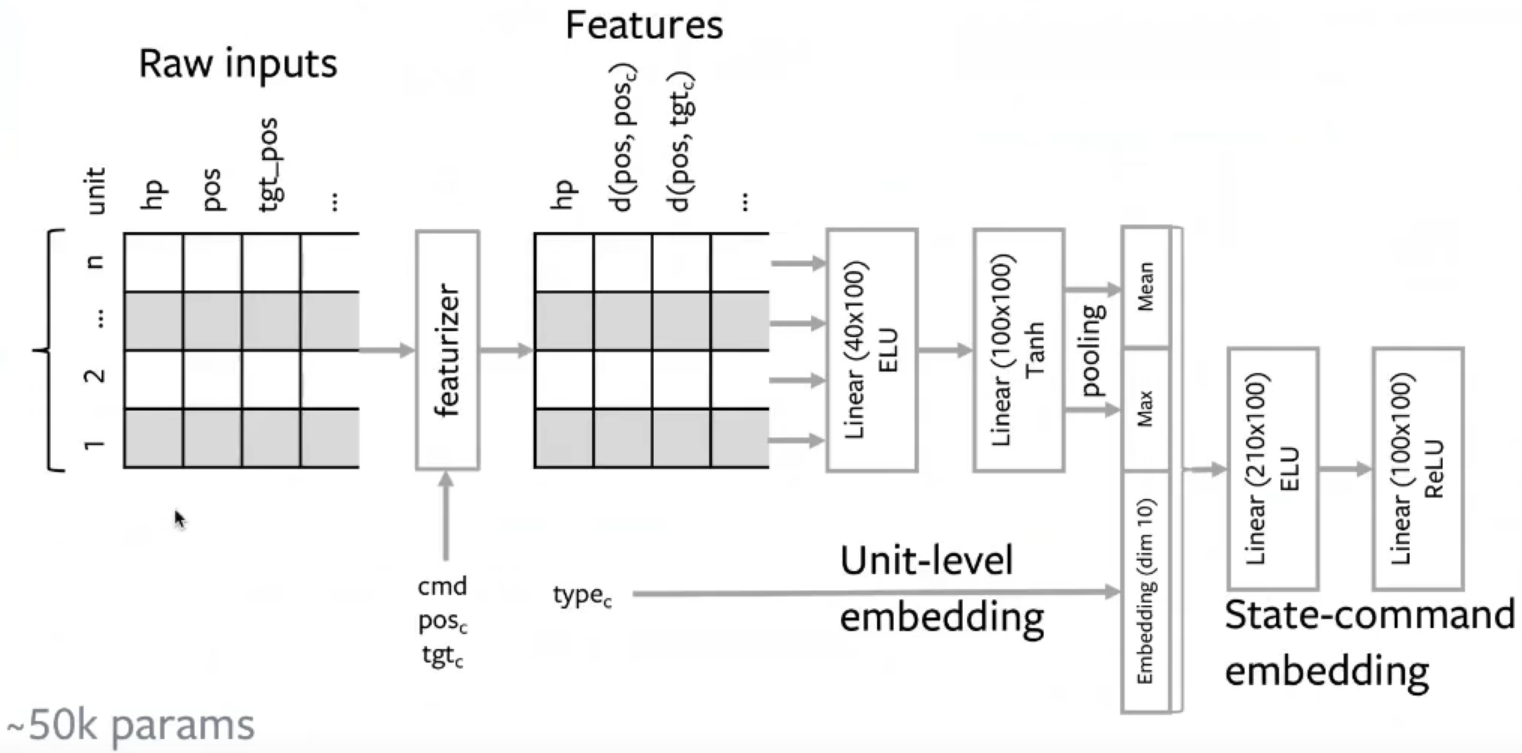
\includegraphics[width=\linewidth]{./figs/model2}}  

\end{frame}

%%%%%%%%%%%%%%%%%%%%%%%%%%%%%%%%%%%%%%%%%%%%%%%%%%%%%%%%%%%%%%%%%%%%%%%%%

\section{Backprop et zero-order gradient}

\begin{frame}
  \frametitle{Backprop et zero-order gradient}

  \begin{block}{Paramètres ($\theta$, w)}
    Deux types de paramètres :
    \begin{itemize}
    \item $\theta$ pour le NN (50k),
    \item w pour la dernière couche (100).
    \end{itemize}
  \end{block}
  
  \bigskip

  \begin{exampleblock}{Zero-order backprop (ZO)}
    \begin{itemize}
    \item Zero-order: $w_{k+1} = w_k + \frac{R}{t}u_k$
    \item    Backprop   :    $\theta_{k+1}   =    \theta_k   +  backprop_{\phi_{\theta_k}}\left(\frac{R}{t}u_k \odot sign\ \frac{w}{\phi_{\theta_k}(s^t,a^t)}\right)$
    \end{itemize}
  \end{exampleblock}

\end{frame}

%%%%%%%%%%%%%%%%%%%%%%%%%%%%%%%%%%%%%%%%%%%%%%%%%%%%%%%%%%%%%%%%%%%%%%%%%

\begin{frame}
  \frametitle{Intuitivement}

  \centerline{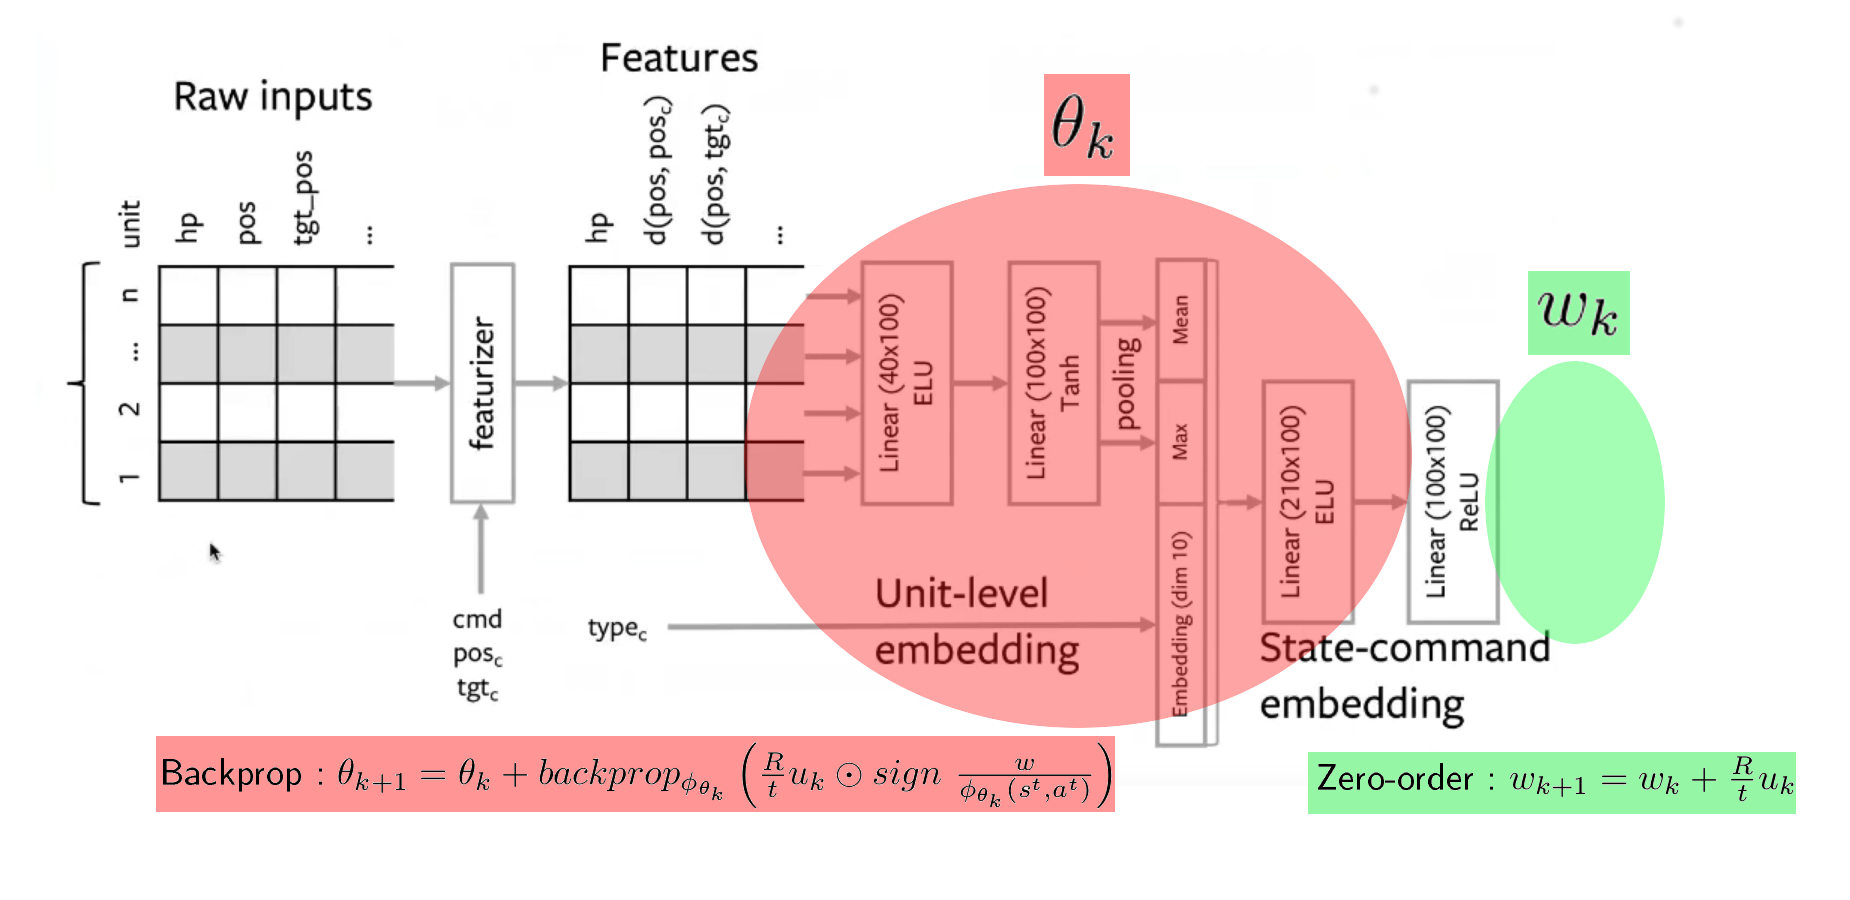
\includegraphics[width=\linewidth]{./figs/mise_a_jour}}  

\end{frame}

%%%%%%%%%%%%%%%%%%%%%%%%%%%%%%%%%%%%%%%%%%%%%%%%%%%%%%%%%%%%%%%%%%%%%%%%%

\section{Résultats expérimentaux}

\begin{frame}
  \frametitle{Résultats expérimentaux}

  \centerline{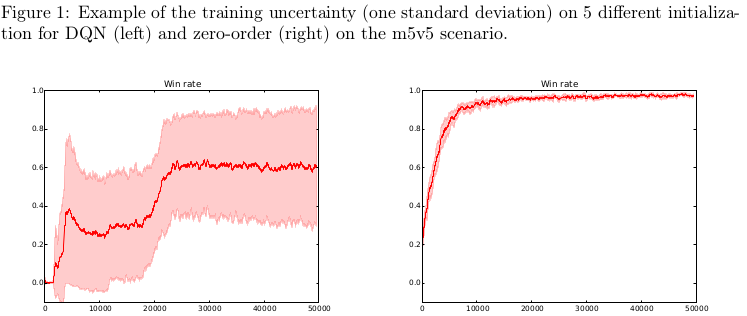
\includegraphics[width=1.1\linewidth]{./figs/results_fig}}

\end{frame}

%%%%%%%%%%%%%%%%%%%%%%%%%%%%%%%%%%%%%%%%%%%%%%%%%%%%%%%%%%%%%%%%%%%%%%%%%

\begin{frame}
  \frametitle{Résultats expérimentaux}

  \centerline{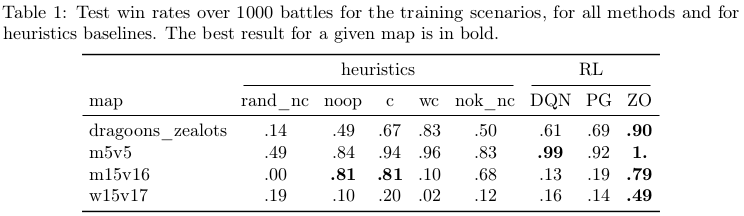
\includegraphics[width=1.1\linewidth]{./figs/results_tab1}}

\end{frame}

%%%%%%%%%%%%%%%%%%%%%%%%%%%%%%%%%%%%%%%%%%%%%%%%%%%%%%%%%%%%%%%%%%%%%%%%%

\begin{frame}
  \frametitle{Résultats expérimentaux}

  \centerline{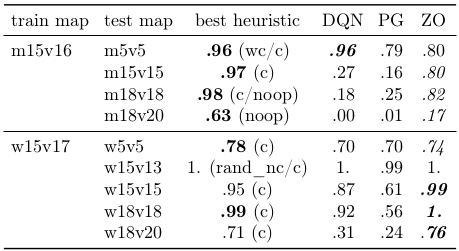
\includegraphics[width=0.7\linewidth]{./figs/results_tab2}}

\end{frame}

%%%%%%%%%%%%%%%%%%%%%%%%%%%%%%%%%%%%%%%%%%%%%%%%%%%%%%%%%%%%%%%%%%%%%%%%%

\begin{frame}
  \frametitle{Résultats expérimentaux}

  \centerline{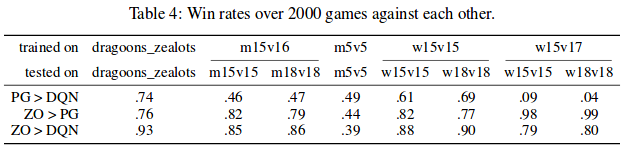
\includegraphics[width=1.1\linewidth]{./figs/winrate}}

\end{frame}

%%%%%%%%%%%%%%%%%%%%%%%%%%%%%%%%%%%%%%%%%%%%%%%%%%%%%%%%%%%%%%%%%%%%%%%%%

\section{Perspectives}

\begin{frame}
  \frametitle{Perspectives}

  \begin{exampleblock}{}
    \begin{itemize}
    \item ConvNet 2D pour apprendre les formes.
      \medskip
    \item Fusion de RL et d'exemples humains.
      \medskip
    \item Hierarchical  RL  pour   apprendre  des  concepts  (fuites, $\ldots$)
    \end{itemize}
  \end{exampleblock}
  
\end{frame}


\end{document}